\chapter{Evaluation}\markright{Chapter 5: Evaluation}\label{sec:evaluation} 
In order to demonstrate the effectiveness of our scheme, we evaluate Accuracy of each defense method compared to the previous scheme.
Accuracy is calculated as:
\begin{equation}
  \mathrm{Accuracy} = \frac{\mathrm{TP}+\mathrm{TN}}{\mathrm{TP} + \mathrm{TN} + \mathrm{FP} + \mathrm{FN}}, 
\end{equation}
where TP, TN, FP, and FN denote the number of True Positive (malwares are regarded as malwares), True Negative (benign files are regarded as benign ones), False Positive (benign files are regarded as malwares), and False Negative (malwares are regarded as benign files), respectively.  

\section{Simulaion parameters}
\tablename~\ref{tab:simulation_parameters} shows our simulation parameters.  
\begin{table}[p]
	\begin{center}
		\caption{Simulation Parameters}
		\label{tab:simulation_parameters} 
		\begin{tabular}{|c|c|} \hline
			The name of parameters & Value\\ \hline \hline
			Benign files & Ubuntu 16.04.3\cite{ubuntu}\\ \hline
			\multirow{2}{*}{\hfill Malwares  \hfill} & IoTPOT\cite{iotpot} \\ 
																							 & VirusTotal\cite{virustotal}\\ \hline
			The number of benign files  & 1,442 \\  \hline
			The number of malwares  &  7,263 \\ \hline
			The AM attack method & White-box \cite{yamafumi} \\ \hline
			\multirow{2}{*}{\hfill The packing tools for OM  \hfill} & UPX\cite{upx} \\ & kiteshield\cite{kiteshield} \\ \hline
			The number of samples  & \multirow{2}{*}{\hfill 800 \hfill} \\  
			in AM-resiliency evaluation & \\ \hline 
			The number of samples  & \multirow{2}{*}{\hfill 1000 \hfill} \\  
			in OM-resiliency evaluation & \\ \hline 
		\end{tabular}
	\end{center}
\end{table} 


We use the benign files from Ubuntu system files \cite{ubuntu} as the begin files.
Meanwhile, malwares are collected from IoTPOT \cite{iotpot} and VirusTotal \cite{virustotal} which is a repository of malware samples for security researchers.
In order to use those samples as inputs for CNN, we convert each sample to the correponding GSI by following the same procedures implemented in \cite{previous}.
In particular, a binary can be reformatted to a sequence whose elements are 8-bit strings.
Then, each string can be converted to a decimal number which can be seen as the value of a one-channel pixel.
After that, we rescale the GSIs to the size of 64*64 such that they can be input to the CNN.
In particular, manipulated malwares for each attack are created with an adversarial technique implemented in \cite{ae} and two packing tools \cite{upx, kiteshield} shown in \tablename~\ref{tab:simulation_parameters}.

In the case of AM-resiliency evaluation, we apply a white-box method as a adversarial technique for AM, where an the adversary knows the training data and the structure of the CNN model since it is currently the mainstream in this reserch field.

In the case of OM-resiliency evaluation, we use two packing tools, called UPX \cite{upx} and kiteshield \cite{kiteshield}, in order for malwares to be obfuscated.
The UPX is a tool which is often utilized mainly for software compression purposes and, according to \cite{pack_research}, the use of it is confirmed in more than 50\% of obfuscated malwares. 
Meanwhile, the kiteshield is a tool which is often utilized mainly for the purpose of encrypting softwares.
Especially, in this evaluation, we prepare three dataset on the basis of which tools to be used for their obfuscation in order to show the versatility in that our scheme is independent of the packing tools.
Two datasets of the three are composed of malwares obfuscated by each packing tooks, UPX and kiteshield, and the other are mixed malwares from those datasets. 

In the evaluation in respective evaluation, some of the samples from total manipulated malwares, 800 samples in AM attack scenario and 1000 samples in OM attack scenario, are picked randomly, then utilized as inputs in order to keep balance between the number of malwares and that of benign ones.

\section{Evaluation of the invalidating adversarial byte sequences against AM attack}
The effectiveness of the proposed method against AM which invalidates adversarial byte sequences with noise removal in the non-valuable pixels is shown in this subsection.
We compare the accuracy of our proposed scheme with that of the previous scheme as shown in \figurename~\ref{fig:evalAM}.
The left graph represents the accuracy of the previous scheme in detecting original malwares, the middle one does that in detecting AM, and the right one does the accuracy of the proposal, where non-valuable pixel values in benign and AM samples are converted to zero.
As shown in \figurename~\ref{fig:evalAM}, the proposed scheme achieves improving the accuracy degraded by AM from 66.1\% to 99.4\%.
Although a slight decrease in detection accuracy is observed compared to the previous scheme and the proposal, the proposal is able to maintain high accuracy.
Thus, the loss of valuable information for classification by removing noise can be considered to be small.
Hence, we conclude that the proposed method against AM, where the non-valuable pixels at runtime are focused on, achieves a robust defense method which can invalidate adversarial techniques in AM.

\section{Evaluation of the method with 1D convolutional filters against OM attack}
\begin{table}[p]
  \begin{center}
    \vspace{-8pt} 
    \caption{The datasets used for the OM-resiliency evaluation}
    \label{tab:evalOM} 
    % \vspace{-8pt} 
    % \hspace{-10pt} 
    \begin{tabular}{|c|c|c|} \hline
      \multirow{2}{*}{\hfill  \hfill} & \multicolumn{2}{c|}{Accuracy}  \\ \cline{2-3} 
					     & Prev. (2D filters) & Prop. (1D filters) \\ \hline \hline
      UPX & 94.8\% & 96.2\% \\ \cline{1-3} 
      kiteshield & 85.0\% & 87.8\% \\ \cline{1-3} 
      mix & 86.2\% & 90.0\% \\ \cline{1-3} 
  \end{tabular}
  \end{center}
\end{table}

The effectiveness of the proposed method with 1D convolutional filters against OM is shown in this subsection.
We compare the accuracy of our proposed scheme using 1D Conv. with that of the previous scheme using 2D Conv. in each dataset as shown in \tablename~\ref{tab:evalOM}.
Compared to 2D Conv. in the previous scheme, the detection accuracy is improved by 1D Conv. in the proposal for all cases.
In the datasets where the both-tools-made OM are mixed in particular, the accuracy improves from 86.2\% to 90.0\%.
According to the result above, we conclude that the proposed method with 1D Conv. against OM achieves a robust defense method with less tool-dependency against OM.

\paragraph{}
In order to observe the relation between the detection accuracy and the filter size of 1D Conv., we evaluate the accuracy varing the filter width.
The 1D Conv. size is changes based on the area of the 2D Conv., which is defined as $S$ in the evaluation, in the previous scheme.
The result is shown in \figurename~\ref{fig:evlOM}, where the red line indicates the accuracy of the proposed scheme and the blue one does that of the previous scheme.
In the range of $1/4S$ to $1.5S$, the accuracy increases as the filter size also increases, and reaches 90.0\% at $1.5S$.
The result suggests that a certain width is necessary to emphasize the appearing order to the CNN model, since the remaining original byte sequences is highly disjoint due to resizing during GSI conversion and compression by obfuscation procedures.
Meanwhile, the accuracy decreases from $1.5S$ to $2.0S$.
We consider that this is caused by the decrease in learning efficiency due to the increase in parameters caused by the expansion of the filter size.

\begin{table}[p]
  \begin{center}
    \caption{\Our evaluation result}
    \label{tab:result} 
    \begin{tabular}{|c|c|c|c|} \hline
      Scheme & Accuracy(\%) & TPR (\%)& FPR (\%) \\ \hline \hline
      \Our scheme & 89.0 & 84.7 & 7.83  \\ \hline
      Previous Scheme & 86.6 & 80.2 & 8.58  \\ \hline 
      SSL certificate based scheme  & 86.6 & 83.2 & 10.1 \\ \hline
      Permission based features & 86.6 & 76.2 & 5.69  \\ \hline
      \Our scheme  & \multirow{2}{*}{89.9} & \multirow{2}{*}{86.3} & \multirow{2}{*}{7.40} \\ 
       \& previous scheme  &  &  &  \\ \hline 
    \end{tabular}
  \end{center}
\end{table} 
\afterpage{\clearpage}
\newpage

\begin{figure}[p]
	% \centering
	% \includegraphics[scale=0.35]{./figure/important_prev_f.pdf}
	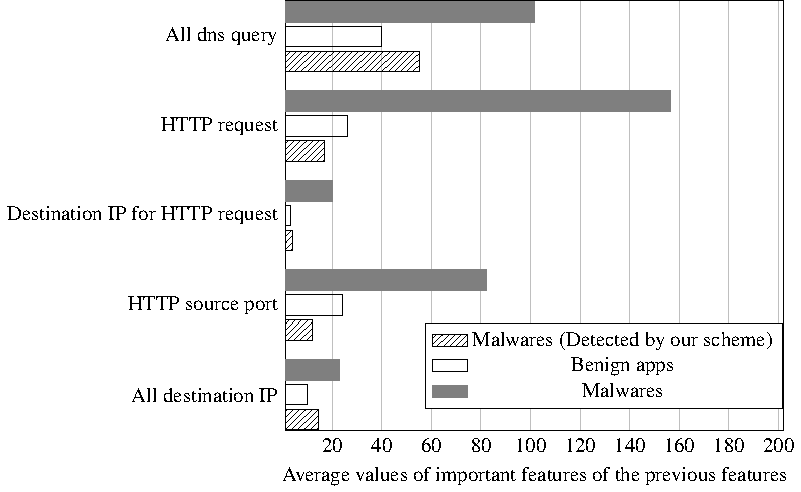
\includegraphics[scale=1.0, bb=10 10 250 250]{./figures/important_prev_f_tikz.pdf}
  \caption{Average values of top 5 important previous features} 
  \label{fig:important_prev_feature}
\end{figure}


\afterpage{\clearpage}
\newpage


